% !TeX root = ../main.tex
\chapter{Vacuum System Design and Experimental Characterization}
\label{chap:vacuum}
\label{chap:design}
% Legacy label retained so existing chapter references continue to resolve.
% Former crawler-design outline retained below until relocation is authorized.
% Requirements and design constraints: traceable requirements table with source,
% target, verification method, and status; confirm dimensions and environment.
% Overall architecture and deployment: labeled system diagram, riser sequence,
% tether/hose routing, operator station, and retrieval strategy.
% Chassis, drivetrain, and traction: wheel geometry, modular assemblies, traction,
% dimensioned CAD, component specifications, materials, and mass properties.
% Distinguish the author's changes from inherited prototype features.
% Electronics and ROS 2: hardware/node diagrams, topics, command/video paths,
% power distribution, software versions, and verified fault behavior.
% The author implemented ROS 2; do not attribute it to Verde's crawler.
% Design tradeoffs: deployment size, traction, suction, power, serviceability,
% and tether effects. Other chapters remain unchanged at the author's request.
\begingroup
\clubpenalty=10000
\widowpenalty=10000

This chapter develops the vacuum-subsystem comparison between one purchased pneumatic conveyor and two units operating in series. The question is whether the second unit increases useful pickup performance enough to justify its additional compressed-air demand. Increased pickup airflow is a hypothesis to be tested. The characterization begins with air-only measurements; subsequent debris tests establish whether any airflow benefit improves material recovery.

The confirmed 12-inch-diameter deployment opening motivates investigating compact units in series instead of simply increasing the size of the onboard conveyor. Fit depends on the complete crawler, including its wheels, equipment, fittings, hose connections, and insertion orientation. A conveyor's nominal diameter alone does not establish deployment clearance. The onboard conveyor is distinct from the external compressor supplying motive air. The opening does not constrain compressor size in this arrangement, and series operation still requires sufficient delivered compressor flow and pressure.

\textbf{Experimental status.} The measurements for this comparison have not yet been supplied. The following procedures are proposed, and the results spaces are reserved for the forthcoming tests. Equipment details that remain unverified are identified explicitly.

\section{Physical Principles and Analytical Framework}
\label{sec:vacuum-principles}

\subsection{Motive Air, Entrainment, and Pickup}
The EXAIR Line Vac uses directed compressed-air jets to entrain air through its inlet and carry material through an open bore toward the discharge \citep{exairLineVacCatalog}. Motive air is the compressed air supplied to those jets. Induced air is the additional air entering through the pickup. The collector must pass the combined air stream while retaining debris. The purchased unit's exact model and geometry must be recorded before applying any model-specific catalog data.

Pickup pressure and pickup flow describe different aspects of operation. Let $p_a$ be local atmospheric pressure and $p_p$ the absolute static pressure at the pickup measurement station. The gauge pressure and positive suction magnitude are defined as
\begin{equation}
 p_{p,g}=p_p-p_a, \qquad S=p_a-p_p=-p_{p,g}.
 \label{eq:pickup-pressure}
\end{equation}
These definitions distinguish negative gauge pressure from a positive vacuum magnitude. A sealed inlet can exhibit suction while admitting essentially no air. Accordingly, a more negative pressure reading alone does not demonstrate better pickup. Airflow must enter the pickup and then transport the target material through the connected path; air-only measurements cannot establish that debris will be entrained or retained.

\subsection{Mass Balance and Compressibility}
For steady air-only operation with negligible leakage and accumulation, conservation of mass gives
\begin{align}
 \dot m_{d,1} &= \dot m_{p,1}+\dot m_{c,A,1}, \\
 \dot m_{d,2} &= \dot m_{p,2}+\dot m_{c,A,2}+\dot m_{c,B,2}.
 \label{eq:conveyor-mass-balance}
\end{align}
Here $p$, $c$, and $d$ denote pickup, compressed-air supply, and discharge; $A$ and $B$ identify the upstream and downstream conveyors. Subscripts 1 and 2 distinguish the single-unit and series configurations. This balance follows the continuity relation $\dot m=\rho A v=\rho Q$, where $\rho$ is local air density, $A$ is flow area, $v$ is mean velocity, and $Q$ is actual volumetric flow \citep{nasaMassFlowChoking}. The series discharge includes both motive streams. Increased discharge flow therefore does not, by itself, establish increased pickup flow.

Volumetric rates at different pressures and temperatures must be converted before comparison. For air approximated as an ideal gas,
\begin{equation}
 \rho=\frac{p}{RT}, \qquad Q_{\mathrm{ref}}=\frac{\dot m}{\rho_{\mathrm{ref}}},
 \label{eq:flow-reference}
\end{equation}
using absolute pressure $p$, absolute temperature $T$, and the specific gas constant $R$ \citep{nasaMassFlowChoking}. Report the reference pressure and temperature whenever a meter provides a normalized volume rate. The comparison will use pickup mass flow and total motive-air mass flow, with pickup volume flow also reported at stated conditions.

The motive jets may involve substantial density changes. In an ideal isentropic nozzle, mass flow reaches a limiting value at sonic conditions; its dependence on supply pressure cannot be represented by an incompressible Bernoulli calculation alone \citep{nasaMassFlowChoking}. Internal jet geometry, mixing losses, and discharge conditions are not sufficiently documented here to predict the purchased conveyor's performance. The analytical framework consequently supports interpretation and measurement checks, while the performance curves must come from experiments.

\subsection{Connected-System Resistance}
For an air-only pipe segment with approximately constant density, the Darcy loss relation and fitting losses give
\begin{equation}
 \Delta p_{\mathrm{loss}}=
 \left(f_D\frac{L}{D}+\sum_j K_j\right)\frac{\rho v^2}{2}.
 \label{eq:vacuum-line-loss}
\end{equation}
Here $f_D$ is the Darcy friction factor, $L$ and $D$ are pipe length and internal diameter, and $K_j$ represents a fitting loss coefficient. Friction factor depends on flow regime and relative roughness \citep{doe1992FluidFlow}. This expression estimates dissipative loss in a specified segment; static-pressure differences can also include velocity and elevation changes. Corrugated hose and uncharacterized fittings require appropriate coefficients or measurements. It is not an internal ejector model, and constant density must not be assumed across the compressed-air expansion or a large pressure change.

The collector introduces additional resistance that depends on its airflow and condition. EXAIR cautions against opposing discharge pressure and undersized exhaust piping \citep{evans2013LineVacBackPressure}. In series operation, the downstream conveyor receives the upstream mixture and adds motive air. Its action changes the pressure seen by the upstream unit, while the collector receives both motive streams. These coupled effects are reasons to measure pickup and discharge conditions rather than adding two catalog suction values. Air-only resistance also excludes particle acceleration, accumulation, and blockage, which must be assessed in debris tests.

\section{Experimental Setup and Measurement Methods}
\label{sec:vacuum-measurements}

\subsection{Apparatus and Information Still Required}
The available project assessment describes two EXAIR Line Vac units conveying toward a collection bag, a pickup pressure location upstream of the units, a discharge pressure location ahead of the bag, and an existing sensor on the compressed-air supply. It does not establish a calibrated inlet-flow measurement. The purchased conveyor will be identified as unit $A$ for the baseline and the added conveyor as unit $B$ for the series test. These identifiers follow flow direction and replace the reversed unit numbering used in the earlier apparatus notes.

The external compressor supplies a regulator and service line leading to the conveyor air ports. The existing supply-pressure sensor will be retained if its range and calibration are suitable; its location must first be checked. A sensor upstream of a restrictive hose or branch does not establish pressure at each unit during operation. Table~\ref{tab:vacuum-setup-status} identifies the setup details needed before the main trials.

\begin{table}[htbp]
\centering
\caption{Vacuum apparatus information to complete before characterization.}
\label{tab:vacuum-setup-status}
\begingroup\small\singlespacing
\renewcommand{\arraystretch}{1.2}
\begin{tabularx}{\textwidth}{@{}p{0.24\textwidth}X@{}}
\toprule
Item & Required record \\
\midrule
Conveyors & Model and unit identifiers, bore, port sizes, flow direction, rated operating limits, and whether both units are the same model. \\
Air supply & Compressor identification and delivered capacity, regulator, service-line dimensions, branch fittings, and actual pressure-tap locations. \\
Conveying path & Pickup geometry, hose internal diameters and lengths, bend layout, elevation, and inter-unit spacing. \\
Collector & Bag or receiver identification, filter area or specification, attachment, and reproducible initial condition. \\
Instrumentation & Sensor models, pressure reference, ranges, calibration, flow-meter method, logging rate, and uncertainty. \\
\bottomrule
\end{tabularx}
\endgroup
\end{table}

The existing pressure-reading code assumes a voltage-to-pressure conversion but does not supply a verified sensor datasheet or calibration record. Those assumptions will not be used as instrument specifications. In particular, extrapolating a positive-pressure sensor's output below its calibrated range cannot establish a valid vacuum measurement.

\subsection{Measurement Stations}
The proposed measurement chain is shown in Figure~\ref{fig:vacuum-test-stations}. The pickup-pressure tap will measure static pressure relative to atmosphere upstream of unit $A$, at a documented location outside the motive-jet region. Supply pressures $p_{c,A,g}$ and $p_{c,B,g}$ will be measured at the respective compressed-air inlet connections while flowing. The discharge tap will measure $p_{d,g}$ before the collector. This last reading represents the connected downstream resistance; it is not a filter-only pressure drop unless taps bracket the filter.

\begin{figure}[htbp]
\centering
\resizebox{\textwidth}{!}{%
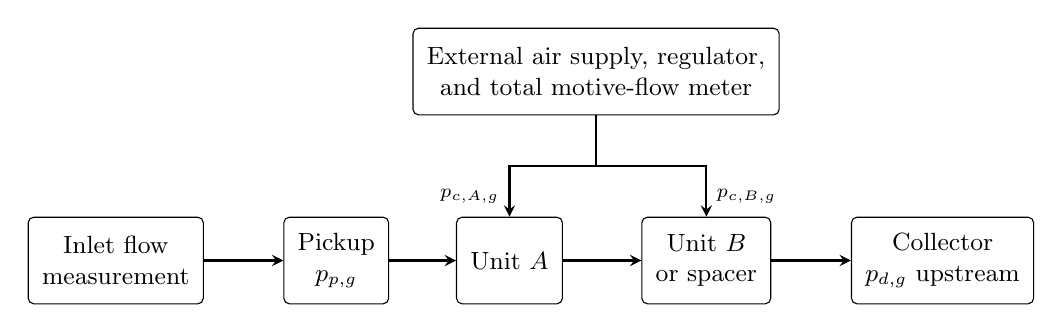
\begin{tikzpicture}[>=stealth,
 box/.style={draw,rounded corners=2pt,align=center,font=\small,minimum height=11mm,inner sep=5pt},
 flow/.style={->,thick}]
\node[box] (meter) at (0,0) {Inlet flow\\measurement};
\node[box] (pickup) at (2.8,0) {Pickup\\$p_{p,g}$};
\node[box] (a) at (5.0,0) {Unit $A$};
\node[box] (b) at (7.5,0) {Unit $B$\\or spacer};
\node[box] (bag) at (10.5,0) {Collector\\$p_{d,g}$ upstream};
\draw[flow] (meter) -- (pickup);
\draw[flow] (pickup) -- (a);
\draw[flow] (a) -- (b);
\draw[flow] (b) -- (bag);
\node[box] (supply) at (6.1,2.4) {External air supply, regulator,\\and total motive-flow meter};
\draw[flow] (supply.south) -- (6.1,1.2) -| node[pos=0.8,left,font=\scriptsize]{$p_{c,A,g}$} (a.north);
\draw[flow] (6.1,1.2) -| node[pos=0.8,right,font=\scriptsize]{$p_{c,B,g}$} (b.north);
\end{tikzpicture}}
\caption[Proposed vacuum characterization measurement stations]{Proposed air-only measurement arrangement, not an as-built drawing. Unit $B$ and its air branch are used only in the series configuration. The inlet meter and required flow-conditioning section must be selected before testing.}
\label{fig:vacuum-test-stations}
\end{figure}

Pickup airflow will be measured upstream of both conveyors so it excludes injected motive air. Total compressed-air consumption will be measured in the common feed dedicated to the conveyors, after regulation and before the branch split, or obtained by summing calibrated branch meters. Other pneumatic users must be isolated or separately measured. The selected meters must accommodate their actual pressure, temperature, flow direction, and operating range. Pressure at the regulator and compressor nameplate capacity are not substitutes for measured consumption.

\subsection{Airflow Conversion and Calibration}
A differential-pressure sensor measures airflow only when paired with a characterized flow element and appropriate pressure taps. A restriction in the pickup line is one candidate; a calibrated direct-reading air-flow meter is another. Orifice metering relates flow to the square root of pressure difference, with coefficients affected by geometry and flow regime \citep{dwyerDifferentialFlow}. For a calibrated restriction in a range where density change across it is negligible, a useful measurement form is
\begin{equation}
 Q_u=C_{\mathrm{cal}}\sqrt{\frac{\Delta p_m}{\rho_u}},
 \qquad \dot m_p=\rho_u Q_u.
 \label{eq:calibrated-pickup-flow}
\end{equation}
The subscript $u$ denotes conditions upstream of the meter, $\Delta p_m$ is the differential across its specified taps, and $C_{\mathrm{cal}}$ includes the flow element's geometry and calibrated coefficient. A constant coefficient is valid only over its verified range. If gas expansion is significant, use the selected meter's compressible-flow relation or calibration rather than Equation~\ref{eq:calibrated-pickup-flow}.

Calibration must cover the anticipated flow range using a suitable reference, with documented pressure, temperature, tap geometry, and straight-run requirements. The sensor's pressure span must resolve the low end without exceeding its upper limit. Density errors and disturbed inlet profiles affect differential-pressure metering \citep{dwyerDifferentialFlow}. The meter also adds resistance, so results must identify the metered configuration; they cannot be presented as unrestricted pickup performance. Leakage between meter and conveyor must be checked before assigning the measured flow to the pickup.

\draftnote{Airflow measurement remains unresolved. Insert the selected meter or restriction, dimensions and tap locations, reference calibration, conversion, validated range, uncertainty, and measured installation loss. Until this is complete, pressure readings must not be reported as airflow.}

\subsection{Uncertainty and Data Reduction}
Each run will retain synchronized pressure and flow records, ambient conditions, configuration identification, and the accepted averaging interval. Independent run means will be used to assess repeatability; samples within one time record will not be counted as independent trials. Calibration, resolution, zero drift, and density correction will be included where applicable.

For a derived result $y=f(x_1,\ldots,x_N)$, first-order propagation gives
\begin{equation}
 u_c^2(y)=\sum_i c_i^2u^2(x_i)
       +2\sum_{i<j}c_i c_j\operatorname{cov}(x_i,x_j),
 \qquad c_i=\frac{\partial f}{\partial x_i}.
 \label{eq:vacuum-uncertainty}
\end{equation}
The covariance terms account for shared inputs and correlated calibration effects \citep{nistUncertaintyPropagation}. Report run count, run-to-run spread, and combined standard uncertainty separately. If expanded uncertainty $U=k u_c$ is reported, state the coverage factor and its justification; a small repeat count does not automatically justify a 95\% interval using $k=2$ \citep{nistExpandedUncertainty}.

\section{Single-Unit Characterization}
\label{sec:single-unit-characterization}
Unit $A$ will establish the baseline with the selected pickup, hose route, and collector. The proposed main matrix uses three supply-pressure levels, two reproducible downstream resistance conditions, and three independent runs per condition: 18 baseline runs. The pressure levels will be selected after checking component ratings and the compressor's sustainable capacity. Numerical setpoints remain to be entered before the main tests.

The two resistance conditions will represent the intended clean collection path and a documented increase in path resistance, such as a second defined hose route. Their exact construction must be fixed in advance and kept identical between configurations. No arbitrary discharge throttling or sealed collector is specified, given the manufacturer's backpressure guidance. If the second condition cannot be justified within the equipment's permitted operation, retain one representative path and state the reduced scope.

Before each run, verify connections, pressure zeros, meter operation, and the collector condition. Set the motive pressure with the conveyor flowing. Record actual inlet pressure, pickup flow, pickup pressure, total motive consumption, and discharge pressure throughout the run. Ambient pressure and temperature will support density correction. Alternate or randomize pressure order within each resistance condition and return to a reference condition to check drift.

Steady operation will be accepted only when successive averaging windows show no systematic trend and changes in the principal pressure and flow channels remain within predefined tolerances. Pilot records will determine the window duration and tolerances from sensor resolution and observed fluctuations. These values, the logging rate, and the run duration must be fixed before the main matrix. Compressor cycling or pressure droop must be recorded; a run that fails the criterion will be identified rather than selectively averaged into a steady result. Independent repeats require resetting and re-establishing the operating condition.

\draftnote{Insert the finalized pressure setpoints, resistance configurations, steady-state tolerances, window and run durations, sampling rate, and completed baseline run log. No single-unit characterization results are available in this draft.}

\section{Two-Unit Series Characterization}
\label{sec:series-characterization}
In the series arrangement, pickup air enters unit $A$, passes through the connecting hose into unit $B$, and then enters the same discharge path and collector. Both conveyors point toward the collector, and both receive motive air from parallel supply branches. They are in series in the conveying path, not in the compressed-air supply. Unit spacing will be defined by the hose length between the outlet connection of $A$ and the inlet connection of $B$; bore, bends, orientation, and fittings will be recorded. One fixed spacing is proposed for the main comparison, not an additional spacing optimization study.

For the baseline, unit $B$ will be removed and replaced with a smooth connector preserving the overall route as closely as practicable. An unpowered second conveyor left in the path is not the single-unit baseline because it introduces its own restriction. Record any residual difference in connector geometry. The collector, pickup, measurement hardware, and downstream resistance conditions will otherwise remain unchanged.

The series matrix repeats the three pressure levels, two resistance conditions, and three independent runs, giving 18 additional runs if both resistance conditions are retained. At each matched-pressure point, the delivered pressure at $A$ and at $B$ will each be brought to the baseline unit's pressure within a stated matching tolerance. Branch regulation or balancing must be selected as needed. Simultaneous measurements at both inlets are required to establish this match; the same regulator setting does not establish equal delivered pressure. If compressor capacity prevents a match, report the measured pressures and classify the condition separately.

The downstream unit may alter the upstream discharge condition, while additional motive air can increase collector loading. Compare $Q_p$, $S$, total motive consumption, and $p_{d,g}$ together. An inter-unit pressure tap may be added for diagnosis if it can be installed without materially disturbing the flow; it is not essential to the initial comparison. Any increase in outlet airflow must be interpreted through Equation~\ref{eq:conveyor-mass-balance}.

A matched-total-consumption comparison is optional. If stable branch control permits it, reduce the series supply settings until the measured sum of motive-air mass flows matches a selected baseline point. Record both resulting inlet pressures. This addresses performance under a common air budget and is distinct from the main matched-pressure comparison. It will be omitted if it requires an extensive additional control or calibration effort.

\draftnote{Insert unit $B$ identification, orientation photograph, inter-unit hose dimensions and spacing, branch layout, pressure-matching tolerance, and series run log. No increase in pickup airflow or suction has yet been established.}

\section{Results, Comparison, and Design Implications}
\label{sec:vacuum-results}
\textbf{Analysis plan; results pending.} The following comparisons will be completed after the measurements are collected and checked. No performance curve, numerical improvement, or preferred unit count is assigned at this stage.

\subsection{Performance Curves and Air Demand}
For each resistance condition, plot pickup airflow, suction magnitude, and total compressed-air mass flow against measured delivered supply pressure. Show both configurations with individual run means and uncertainty, identifying series points where the two supply pressures were not adequately matched. Plot pickup flow against total motive consumption as a second view of the tradeoff. Discharge-pressure records will help identify changes associated with the downstream path.

At comparable conditions, define
\begin{equation}
 \Delta Q_p=Q_{p,2}-Q_{p,1}, \qquad
 \Delta\dot m_c=\dot m_{c,2}-\dot m_{c,1}, \qquad
 E=\frac{\dot m_p}{\dot m_c}.
 \label{eq:vacuum-comparison}
\end{equation}
Here $\dot m_c$ is total motive consumption, and $E$ is an induced-to-motive air mass-flow ratio, not thermodynamic efficiency or debris recovery efficiency. Compare volume rates at common stated conditions. Report uncertainty on differences and ratios, accounting for shared calibration. Relative improvement may be reported only when the baseline value is sufficiently above zero to make the ratio meaningful. Curves will describe the measured range without extrapolating an optimum.

\draftnote{Results space: insert single-unit and series performance curves with uncertainty, the condition-by-condition comparison table, supply-pressure stability records, and observations of downstream resistance. Preserve failed or excluded runs and explain their treatment.}

\subsection{Configuration Selection and Debris Validation}
A useful series benefit requires more than a detectable increase in air-only flow. The change must be practically meaningful for pickup, compatible with compressor capacity, and achievable within the complete deployment envelope. The minimum useful improvement and acceptable air demand will be defined before the main comparison. If the second unit offers little or no benefit, or its additional demand outweighs the benefit, the single-unit arrangement remains a valid outcome. The comparison may also remain inconclusive if uncertainty is too large.

Subsequent tests will use known masses of the target dust and sand-type debris, with specified particle size, moisture, pickup geometry, standoff, path, duration, and collector condition. Chapter~\ref{chap:methods} defines these recovery trials and their integration with crawler operation. They will distinguish material recovered in the collector from material left on the floor or retained in the conveying path. Compressed-air use per recovered mass and blockage occurrence will supplement recovery efficiency and collection rate. Airflow improvement will not be equated with improved cleaning efficiency without this evidence.

\draftnote{Results space: state the supported air-only configuration decision and its uncertainty, then link the subsequent debris results in Chapter~\ref{chap:results}. Record any revision to that decision after practical recovery testing.}
\par
\endgroup
